% Physics experiment report
% 18/Nov/2016

\documentclass[a4paper,10pt,notitlepage]{article}

\usepackage{CJKutf8}
\usepackage{amsmath}
\usepackage{indentfirst}
\usepackage{graphicx}
\usepackage{longtable}

\setlength{\parindent}{2em} 

\begin{CJK*}{UTF8}{gbsn}
\begin{document}

\title{测量金属杨氏模量实验报告}
\author{秦光辉\ 9组3号}
\maketitle

\section{实验数据处理}

\subsection{CCD成像系统测金属杨氏模量}

	使用千分尺测量金属丝的直径, 得到不同位置处的直径, 一共测量十次, 结果见表一. 其中千分尺的允差为0.01mm, 零点为
	
\begin{equation*}
	x_0 = -0.001mm
\end{equation*}

\begin{center}

	\begin{longtable}{|c|c|c|c|c|c|}
	\caption{金属丝直径} \\
	\hline
	n & 1 & 2 & 3 & 4 & 5 \\
	\hline
	d/mm & 0.320 & 0.321 & 0.325 & 0.325 & 0.326 \\
	\hline
	\hline
	n & 6 & 7 & 8 & 9 & 10 \\
	\hline
	d/mm & 0.324 & 0.323 & 0.324 & 0.328 & 0.322 \\
	\hline
	\end{longtable}

\end{center}

	可以计算得直径的均值和不确定度为
	
\begin{align*}
	\bar{d} &= 0.3238 mm \\
	\sigma_{\bar{d}} &= \frac{\sum_{i = 1}^{n}d_i}{\sqrt{n(n-1)}} = 7.5 \times 10^{-4} mm \\
	\sigma_d &= \sqrt{\frac{e^2}{3} + \sigma_d ^ 2} = 6 \times 10^{-3} mm \\
	d &= 0.324 \pm 0.006 mm
\end{align*}

	考虑螺旋测微计零点偏移, 得到
	
\begin{align*}
	d &= 3.25 \pm 0.06 \times 10^{-4} m
\end{align*}

	测量金属丝的长度, 共测量一次, 其允差为0.15cm, 可以得到
	
\begin{align*}
	l_i &= 17.02 cm \\
	l_f &= 95.60 cm \\
	l &= 78.58 cm \\
	\sigma_l &= \sqrt{\frac{e^2}{3} + \frac{e^2}{3}} = 1.22 \times 10^{-3} m \\
	l &= 7.86 \pm 0.02 \times 10 ^ {-1} m
\end{align*}

	砝码的质量见表二. 仪器允差为0.01g. \\
	
\begin{center}

	\begin{longtable}{|c|c|c|c|c|c|}
	\caption{CCD法测量金属丝杨氏模量砝码重量}\\
	\hline
	n & 1 & 2 & 3 & 4 & 5 \\
	\hline
	m/g & 200.38 & 200.36 & 200.17 & 200.08 & 199.97 \\
	\hline
	\hline
	n & 6 & 7 & 8 & 9 &  \\
	\hline
	m/g & 200.03 & 200.08 & 200.84 & 199.80 &  \\
	\hline
	\end{longtable}

\end{center}

	并且可以得到 \\

\begin{align*}
	\bar{m} &= 200.19 g \\
	\sigma_m &= \frac{\sum_{i = 1}^{n}m_i}{\sqrt{n(n-1)}} = 0.101256 g \\
\end{align*}

	仪器误差非常小, 忽略不计. 在上面的测量中可以看到金属丝长度的相对不确定度大约为0.25\%, 金属丝直径的相对不确定度更是达到了1.8\%, 这里我们可以看出砝码的质量相对不确定度非常小, 仅为0.05\%, 完全可以忽略不计. \\
	
	金属丝长度在每次测量中的伸长量如表三所示. 其中仪器允差为0.05mm. \\
	
\begin{center}

	\begin{longtable}{|c|c|c|c|c|c|}
	\caption{CCD实验中金属丝伸长量数据表} \\
	\hline
	n & 0 & 1 & 2 & 3 & 4 \\
	\hline
	x/mm & 2.25 & 2.39 & 2.51 & 2.64 & 2.76 \\
	\hline
	$x'$/mm & 2.24 & 2.37 & 2.51 & 2.64 & 2.76 \\
	\hline
	$\bar{x}$/mm & 2.25 & 2.38 & 2.51 & 2.64 & 2.76 \\
	\hline
	\hline
	n & 5 & 6 & 7 & 8 & 9 \\
	\hline
	x/mm & 2.88 & 3.00 & 3.11 & 3.23 & 3.35 \\
	\hline
	$x'$/mm & 2.87 & 2.99 & 3.10 & 3.23 & 3.35 \\
	\hline
	$\bar{x}$/mm & 2.88 & 3.00 & 3.105 & 3.23 & 3.35 \\
	\hline
	\end{longtable}

\end{center}

\subsubsection{使用最小二乘法拟合直线}

	可以计算得到如下结论. \\

\begin{align*}
	k &= 0.121515 mm \\
	b &= 2.26218 mm \\
	r &= 0.999672 \\
	\sigma_k &= \frac{\sigma}{\sqrt{\sum_{i = 1}^n (x_i - \bar{x})^2}} \\
	\sigma &= \frac{e}{\sqrt{3}} = 0.0288 mm \\
	\sigma_k &= 3.178 \times 10^{-3} \\
	k &= 0.122 \pm 0.004 mm
\end{align*}

	拟合直线见图一. \\
	
\begin{figure}
\centering
	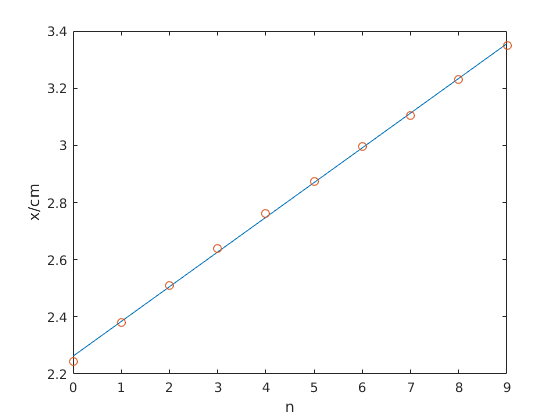
\includegraphics[scale=0.7]{ym1.png}
	\caption{CCD法测杨氏模量线性拟合直线}
\end{figure}

	这样我们可以得到
	
\begin{align*}
	E &= \frac{4mgl}{\pi d^2k} = 1.53748 \times 10^{11} Pa \\
	\delta_E &= E \times \sqrt{(\frac{\sigma_{k}}{k})^2 + (\frac{\sigma_{d}}{d})^2\times 2 + (\frac{\sigma_{m}}{m})^2 + (\frac{\sigma_{l}}{l})^2} = 0.06 \times 10^{11} Pa 
\end{align*}

	可以得到E的最终结果为
	
\begin{align*}
	E &= 1.54 \pm 0.06 \times 10^{11} Pa
\end{align*}

\subsubsection{使用逐差法处理数据}

\begin{center}

	\begin{longtable}{|c|c|c|c|c|c|}
	\caption{CCD实验中金属丝伸长量数据表} \\
	\hline
	n & 0 & 1 & 2 & 3 & 4 \\
	\hline
	x/mm & 2.25 & 2.39 & 2.51 & 2.64 & 2.76 \\
	\hline
	$x'$/mm & 2.24 & 2.37 & 2.51 & 2.64 & 2.76 \\
	\hline
	$\bar{x}$/mm & 2.245 & 2.38 & 2.51 & 2.64 & 2.76 \\
	\hline
	n & 5 & 6 & 7 & 8 & 9 \\
	\hline
	x/mm & 2.88 & 3.00 & 3.11 & 3.23 & 3.35 \\
	\hline
	$x'$/mm & 2.87 & 2.99 & 3.10 & 3.23 & 3.35 \\
	\hline
	$\bar{x}$/mm & 2.875 & 2.995 & 3.105 & 3.23 & 3.35 \\
	\hline
	$x_{i+5} - x_i$ & 0.63 & 0.62 & 0.60 & 0.59 & 0.59 \\
	\hline
	\end{longtable}
	
\end{center}
	
	设
	
\begin{align*}
	\Delta x &= \frac{\sum_{i = 5}^9x_i - \sum_{i = 0}^4x_i}{25} 
\end{align*}

	由仪器允差带来的不确定度为
	
\begin{align*}
	\sigma_{\Delta x} &= \sqrt{(\frac{e}{\sqrt{3}})^2 \times 10} \times \frac{1}{25} = 3.65 \times 10^{-3} mm \\
\end{align*}

	多次测量的随机误差为
	
\begin{align*}
	\sigma_{\bar{\Delta x}} &= \sqrt{\frac{\sum_{i = 0}^5 ((x_{i+5} - x_i) - \overline{(x_{i+5} - x_i)}) ^ 2}{n ( n - 1)}} = 2 \times 10^{-3} mm\\
\end{align*}

	合成的不确定度为
	
\begin{align*}
	\sigma_{\Delta x}' &= \sqrt{\sigma_{\Delta x}^2 + \sigma_{\bar{\Delta x}}^2} = 5 \times 10^{-3} mm \\
\end{align*}

	这样我们可以得到
	
\begin{align*}
	E &= \frac{4mgl}{\pi d^2\Delta x} = 1.53748 \times 10^{11} Pa \\
	\delta_E &= E \times \sqrt{(\frac{\sigma_{\Delta x}}{\Delta x})^2 + (\frac{\sigma_{d}}{d})^2\times 2 + (\frac{\sigma_{m}}{m})^2 + (\frac{\sigma_{l}}{l})^2} = 0.06 \times 10^{11} Pa 
\end{align*}

	可以得到E的最终结果为
	
\begin{align*}
	E &= 1.54 \pm 0.06 \times 10^{11} Pa
\end{align*}

\subsection{光杠杆法测金属的杨氏模量}

	测量金属质量的数据见表五. \\

\begin{center}

	\begin{longtable}{|c|c|c|c|c|c|c|}
	\caption{光杠杆法测金属杨氏模量金属质量数据} \\
	\hline
	n & 1 & 2 & 3 & 4 & 5 & 6 \\
	\hline
	m/g & 199.84 & 200.03 & 199.71 & 199.69 & 199.79 & 199.91 \\
	\hline
	\hline
	n & 7 & 8 & 9 & 10 & 11 &  \\
	\hline
	m/g & 199.83 & 200.10 & 199.62 & 199.72 & 199.85 &  \\
	\hline
	\end{longtable}

\end{center}

	得到
	
\begin{align*}
	\bar{m} &= 199.82g \\
\end{align*}
	
	测量金属丝长度, 得到
	
\begin{align*}
	l_i &= 1.02 cm \\
	l_f &= 141.60 cm \\
	l &= 140.58 cm 
\end{align*}

	测量钢尺到镜面的距离, 有
	
\begin{align*}
	L_i &= 53.19 cm \\
	L_f &= 130.40 cm \\
	L &= 77.21 cm 
\end{align*}

	将镜面的底边和顶角用力压在纸面上留下痕迹, 用游标卡尺测得顶点到底边的距离为
	
\begin{align*}
	D &= 9.145 cm 
\end{align*}

	加砝码再卸砝码, 得到两组数据, 如表六. \\
	
\begin{center}

	\begin{longtable}{|c|c|c|c|c|c|c|}
	\caption{光杠杆测金属杨氏模量实验数据表} \\
	\hline
	n & 0 & 1 & 2 & 3 & 4 & 5 \\
	\hline
	$x$/cm & 10.52 & 10.90 & 11.20 & 11.69 & 11.98 & 12.34 \\
	\hline
	$x'$/cm & 10.85 & 11.05 & 11.41 & 11.71 & 12.05 & 12.40 \\
	\hline
	$\bar{x}$/cm & 10.68 & 10.98 & 11.30 & 11.70 & 12.02 & 12.37 \\
	\hline
	\hline
	n & 6 & 7 & 8 & 9 & 10 & 11 \\
	\hline
	$x$/cm & 12.65 & 13.09 & 13.41 & 13.79 & 14.11 & 14.42 \\
	\hline
	$x'$/cm & 12.78 & 13.13 & 13.47 & 13.80 & 14.08 & 14.42 \\
	\hline
	$\bar{x}$/cm & 12.72 & 13.11 & 13.44 & 13.79 & 14.09 & 14.42 \\
	\hline
	\end{longtable}

\end{center}
	
	使用最小二乘法处理数据, 得到斜率为
	
\begin{align*}
	k &= 0.345734 cm 
\end{align*}

	拟合直线如图二. \\
	
\begin{figure}[h]
\centering
	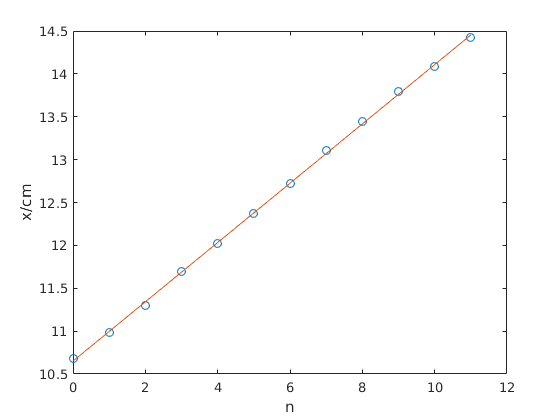
\includegraphics[scale=0.7]{ym2.png}
	\caption{光杠杆法测量金属杨氏模量拟合直线}
\end{figure}

	金属丝直径数据见表七. \\

\begin{center}

	\begin{longtable}{|c|c|c|c|c|c|}
	\caption{金属丝直径} \\
	\hline
	n & 1 & 2 & 3 & 4 & 5 \\
	\hline
	d/mm & 0.324 & 0.322 & 0.323 & 0.325 & 0.326 \\
	\hline
	\hline
	n & 6 & 7 & 8 & 9 & 10 \\
	\hline
	d/mm & 0.324 & 0.323 & 0.323 & 0.328 & 0.324 \\
	\hline
	\end{longtable}

\end{center}

	可以计算得直径的均值为
	
\begin{align*}
	\bar{d} &= 0.325 mm 
\end{align*}

	可以算出金属杨氏模量为
	
\begin{align*}
	E &= \frac{8mglL}{\pi d^2 D k} = 1.54 \times 10^{11} Pa
\end{align*}
	
\subsection{梁的弯曲实验}

	使用螺旋测微计测量板的厚度, 数据如表八. \\
	
\begin{center}

	\begin{longtable}{|c|c|c|c|c|c|}
	\caption{梁的厚度数据表} \\
	\hline
	n & 1 & 2 & 3 & 4 & 5 \\
	\hline
	d/mm & 1.504 & 1.500 & 1.502 & 1.509 & 1.500 \\
	\hline
	\hline
	n & 6 & 7 & 8 & 9 & 10 \\
	\hline
	d/mm & 1.499 & 1.498 & 1.505 & 1.504 & 1.507 \\
	\hline
	\end{longtable}

\end{center}

	螺旋测微计零点为-0.001mm, 得到d的均值为
	
\begin{align*}
	\bar{d} &= 1.504 mm
\end{align*}

	用游标卡尺测梁的宽度, 零点为0.00 mm, 得到如表九的数据. \\
	
\begin{center}

	\begin{longtable}{|c|c|c|c|c|c|}
	\caption{梁的宽度实验数据表} \\
	\hline
	n & 1 & 2 & 3 & 4 & 5 \\
	\hline
	a/mm & 14.90 & 14.95 & 14.90 & 14.85 & 15.00 \\
	\hline
	\hline
	n & 6 & 7 & 8 & 9 & 10 \\
	\hline
	a/mm & 15.05 & 15.00 & 14.90 & 15.00 & 14.95 \\
	\hline
	\end{longtable}

\end{center}

	可得宽度a的平均值为

\begin{align*}
	\bar{a} &= 14.95 mm
\end{align*}

	砝码的质量测量如表十. \\
	
\begin{center}

	\begin{longtable}{|c|c|c|c|c|c|c|}
	\caption{梁的弯曲实验中砝码质量测量数据表} \\
	\hline
	n & 1 & 2 & 3 & 4 & 5 & 6 \\
	\hline
	m/g & 199.91 & 199.74 & 200.03 & 199.78 & 199.77 & 200.14 \\
	\hline
	\end{longtable}

\end{center}

	砝码的平均质量为
	
\begin{align*}
	\bar{m} &= 199.90 g
\end{align*}

	实验中梁的高度和砝码数量的关系如表十一. \\
	
\begin{center}

	\begin{longtable}{|c|c|c|c|c|c|c|c|}
	\caption{梁的高度随砝码数量增加变化关系表} \\
	\hline
	n & 0 & 1 & 2 & 3 & 4 & 5 & 6 \\
	\hline
	$x$/mm & 41.866 & 40.612 & 39.318 & 38.021 & 36.698 & 35.408 & 34.033 \\
	\hline
	$x'$/mm & 41.892 & 40.558 & 39.250 & 27.913 & 36.608 & 35.296 & 33.961 \\
	\hline
	$\bar{x}$/mm & 41.879 & 40.585 & 39.284 & 37.967 & 36.653 & 35.352 & 33.997 \\
	\hline
	\end{longtable}

\end{center}

	用最小二乘法拟合曲线, 有
	
\begin{align*}
	|k| &= 1.3123mm
\end{align*}

	拟合图线见图三. \\
	
\begin{figure}[h]
\centering
	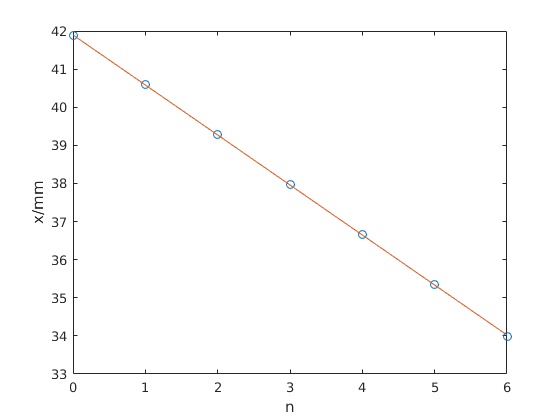
\includegraphics[scale=0.7]{ym3.png}
	\caption{梁的高度随砝码数量增加变化拟合直线}
\end{figure}

	测量两个刀口之间的距离, 有
	
\begin{align*}
	L_i &= 31.19 cm \\
	L_f &= 5.00 cm \\
	L &= 27.19 cm 
\end{align*}

	最后可以计算得到梁的杨氏模量为

\begin{align*}
	E = \frac{mgL^3}{4dh^3k} = 1.476 \times 10^{11} Pa
\end{align*}

\section{讨论与分析}

\subsection{开始加第一、二个砝码时 r 的变化量大于正常的变化量, 为什么?}

\begin{enumerate}
	\item 实验中的钢丝其实并不非常直, 触摸之后可以发现其实它有一些微小的折痕. 在测量过程中, 加上砝码可以把它拉直.
	\item 钢丝的卡口可能有松动.
	\item 砝码可能质量有高有低.
\end{enumerate}

\subsection{在上述情况下 r 的变化量小于正常的变化量, 为什么?}

\begin{enumerate}
	\item 可能钢丝没有完全竖直, 中间有摩擦力作用. 这个力在重量增加之后影响会变小.
	\item 钢丝的截面积在没有外力作用的时候相对较大, 这时候弹性系数小.
	\item 砝码可能质量有高有低.
\end{enumerate}

\section{思考和感悟}

	我觉得这个实验是特别有意思的一个实验, 特别是光杠杆测量金属的杨氏模量实验. 这么精巧的实验, 做出来特别有成就感. 这个实验和卡文迪许的实验非常类似, 都是用光路来放大微小的位移量. 类似的还有很多, 比如可以用电阻的改变测量温度的变化(铂电阻温度计), 而电阻的改变又可以用非平衡电桥测量等等. 一些物理量可以转换为另外一些物理量测量, 这样可以使得原来不好测量的物理量变得容易测量, 特别小的物理量可以变得很大, 而且这种转换往往是跨学科的. 这种精妙的思路让我赞叹不已!
	
\end{CJK*}
\end{document}
